\chapterbegin

\section[Procedures for Aerodrome Control Service]{PROCEDURES FOR AERODROME CONTROL SERVICE}

\subsection[Functions of aerodrome control towers]{FUNCTIONS OF AERODROME CONTROL TOWERS}

\subsubsection{General}

\begin{enumerate}
    \item Aerodrome control towers shall issue information and clearances to aircraft under their control to achieve a safe, orderly and expeditious flow of air traffic on and in the vicinity of an aerodrome with the object of preventing collision(s) between:

    \begin{enumalph}
        \item aircraft flying within the designated area of responsibility of the control tower, including the aerodrome traffic circuits;
        \item aircraft operating on the manoeuvring area;
        \item aircraft landing and taking off;
        \item aircraft and vehicles operating on the manoeuvring area;
        \item aircraft on the manoeuvring area and obstructions on that area.
    \end{enumalph}

    \item Aerodrome controllers shall maintain a continuous watch on all flight operations on and in the vicinity of an aerodrome as well as vehicles and personnel on the manoeuvring area. Watch shall be maintained by visual observation, augmented in low visibility conditions by an ATS surveillance system when available. Traffic shall be controlled in accordance with the procedures set forth herein and all applicable traffic rules specified by the appropriate ATS authority. If there are other aerodromes within a control zone, traffic at all aerodromes within such a zone shall be coordinated so that traffic circuits do not conflict.
    %References
    \note{Provisions for the use of an ATS surveillance system in the aerodrome control service are contained in Chapter 8, Section 8.10.}

    \item The functions of an aerodrome control tower may be performed by different control or working positions, such as:

    \begin{enumalph}
        \item aerodrome controller, normally responsible for operations on the runway and aircraft flying within the area of responsibility of the aerodrome control tower;
        \item ground controller, normally responsible for traffic on the manoeuvring area with the exception of runways;
        \item clearance delivery position, normally responsible for delivery of start-up and ATC clearances to departing IFR flights.
    \end{enumalph}

    \item Where parallel or near-parallel runways are used for simultaneous operations, individual aerodrome controllers should be responsible for operations on each of the runways.
\end{enumerate}

%Numbering
%7.1.2
%7.1.3

\subsection[Selection of runway-in-use]{SELECTION OF RUNWAY-IN-USE}

\begin{enumnoss}
    \item The term ``runway-in-use" shall be used to indicate the runway or runways that, at a particular time, are considered by the aerodrome control tower to be the most suitable for use by the types of aircraft expected to land or take off at the aerodrome.
    \note{Separate or multiple runways may be designated runway-in-use for arriving aircraft and departing aircraft.}
    \item Normally, an aircraft will land and take off into wind unless safety, the runway configuration, meteorological conditions and available instrument approach procedures or air traffic conditions determine that a different direction is preferable. In selecting the runway-in-use, however, the unit providing aerodrome control service shall take into consideration, besides surface wind speed and direction, other relevant factors such as the aerodrome traffic circuits, the length of runways, and the approach and landing aids available.
    \item A runway for take-off or landing, appropriate to the operation, may be nominated for noise abatement purposes, the objective being to utilize whenever possible those runways that permit aeroplanes to avoid noise-sensitive areas during the initial departure and final approach phases of flight.
    \item Runways should not be selected for noise abatement purposes for landing operations unless they are equipped with suitable glide path guidance, e.g. ILS, or a visual approach slope indicator system for operations in visual meteorological conditions.
    \item A pilot-in-command, prompted by safety concerns, can refuse a runway offered for noise-pref\-er\-en\-tial reasons.
    \item Noise abatement shall not be a determining factor in runway nomination under the following circumstances:

    \begin{enumalph}
        \item if the runway surface conditions are adversely affected (e.g. by snow, slush, ice, water, mud, rubber, oil or other substances);
        \item for landing in conditions:

        \begin{enumarab}
            \item when the ceiling is lower than 500 ft above aerodrome elevation, or the visibility is less than 1 900 m; or
            \item when the approach requires use to be made of vertical minima greater than 300 ft above aerodrome elevation and:

            \begin{enumroman}
                \item the ceiling is lower than 800 ft above aerodrome elevation; or
                \item the visibility is less than 3 000 m;
            \end{enumroman}
        \end{enumarab}

        \item for take-off when the visibility is less than 1 900 m;
        \item when wind shear has been reported or forecast or when thunderstorms are expected to affect the approach or departure; and
        \item when the crosswind component, including gusts, exceeds 15 kt, or the tailwind component, including gusts, exceeds 5 kt.
    \end{enumalph}
\end{enumnoss}

\subsection[Initial call to aerodrome control tower]{INITIAL CALL TO AERODROME CONTROL TOWER}

For aircraft being provided with aerodrome control service, the initial call shall contain:

\begin{enumalph}
    \item designation of the station being called;
    \item call sign and, for aircraft in the heavy wake turbulence category, the word ``Heavy";
    \item position; and
    \item additional elements, as required by the appropriate ATS authority.
\end{enumalph}

%References
\note{See also Chapter 4, 4.11.3, for aircraft in the air, making the first call to the aerodrome tower.}

\subsection[Information to aircraft by aerodrome control towers]{INFORMATION TO AIRCRAFT BY AERODROME CONTROL TOWERS}

\subsubsection{Information related to the operation of aircraft}

\begin{enumempty}[labelindent=\parindent]
    %References
    \item \note{See Chapter 11, 11.4.3, regarding flight information messages.}
\end{enumempty}

\begin{enumeratesc}
    \item \textsc{Start-up time procedures}
    \begin{enumerate}
        \item When so requested by the pilot prior to engine start, an expected take-off time should be given, unless engine start-up time procedures are employed.
        \item Start-up time procedures should be implemented where necessary to avoid congestion and excessive delays on the manoeuvring area or when warranted by ATFM regulations. Start-up time procedures should be contained in local instructions, and should specify the criteria and conditions for determining when and how start-up times shall be calculated and issued to departing flights.
        \item When an aircraft is subject to ATFM regulations, it should be advised to start up in accordance with its allocated slot time.
        \item When the delay for a departing aircraft is anticipated to be less than a time period specified by the appropriate ATS authority, an aircraft should be cleared to start up at its own discretion.
        \item When the delay for a departing aircraft is anticipated to exceed a time period specified by the appropriate ATS authority, the aerodrome control tower should issue an expected start-up time to an aircraft requesting start-up.
        \item A start-up clearance shall only be withheld under circumstances or conditions specified by the appropriate ATS authority.
        \item If a start-up clearance is withheld, the flight crew shall be advised of the reason.
    \end{enumerate}

    \item \textsc{Aerodrome and meteorological information}
    \begin{enumerate}
        \item \label{7.4.1.2.1} Prior to taxiing for take-off, aircraft shall be advised of the following elements of information, in the order listed, with the exception of such elements which it is known the aircraft has already received:
        
        \begin{enumalph}
            \item the runway to be used;
            \item the surface wind direction and speed, including significant variations therefrom;
            \item the QNH altimeter setting and, either on a regular basis in accordance with local arrangements or if so requested by the aircraft, the QFE altimeter setting;
            \item the air temperature for the runway to be used, in the case of turbine-engined aircraft;
            \item the visibility representative of the direction of take-off and initial climb, if less than 10 km, or, when applicable, the RVR value(s) for the runway to be used;
            \item the correct time.
        \end{enumalph}

        %References
        \note{The meteorological information listed above is to follow the criteria used for meteorological local routine and special reports, in accordance with Chapter 11, 11.4.3.2.2 to 11.4.3.2.3.}

        \item Prior to take-off aircraft shall be advised of:
        
        \begin{enumalph}
            \item any significant changes in the surface wind direction and speed, the air temperature, and the visibility or RVR value(s) given in accordance with \ref{7.4.1.2.1};
            \item significant meteorological conditions in the take-off and climb-out area, except when it is known that the information has already been received by the aircraft.
        \end{enumalph}

        \note{Significant meteorological conditions in this context include the occurrence or expected occurrence of cumulonimbus or thunderstorm, moderate or severe turbulence, wind shear, hail, moderate or severe icing, severe squall line, freezing precipitation, severe mountain waves, sandstorm, duststorm, blowing snow, tornado or waterspout in the take-off and climb-out area.}

        \item Prior to entering the traffic circuit or commencing its approach to land, an aircraft shall be provided with the following elements of information, in the order listed, with the exception of such elements which it is known the aircraft has already received:

        \begin{enumalph}
            \item the runway to be used;
            \item the surface wind direction and speed, including significant variations therefrom;
            \item the QNH altimeter setting and, either on a regular basis in accordance with local arrangements or if so requested by the aircraft, the QFE altimeter setting.
        \end{enumalph}

        %References
        \note{The meteorological information listed above is to follow the criteria used for meteorological local routine and special reports, in accordance with Chapter 11, 11.4.3.2.2 to 11.4.3.2.3.}
    \end{enumerate}

    \item \textsc{Essential local traffic information}
    \begin{enumerate}
        \item Information on essential local traffic shall be issued in a timely manner, either directly or through the unit providing approach control service when, in the judgement of the aerodrome controller, such information is necessary in the interests of safety, or when requested by aircraft.
        \item Essential local traffic shall be considered to consist of any aircraft, vehicle or personnel on or near the manoeuvring area, or traffic operating in the vicinity of the aerodrome, which may constitute a hazard to the aircraft concerned.
        \item Essential local traffic shall be described so as to be easily identified.
    \end{enumerate}

    \item \textsc{Runway incursion or obstructed runway}
    \begin{enumerate}
        \item In the event the aerodrome controller, after a take-off clearance or a landing clearance has been issued, becomes aware of a runway incursion or the imminent occurrence thereof, or the existence of any obstruction on or in close proximity to the runway likely to impair the safety of an aircraft taking off or landing, appropriate action shall be taken as follows:

        \begin{enumalph}
            \item cancel the take-off clearance for a departing aircraft;
            \item instruct a landing aircraft to execute a go-around or missed approach;
            \item in all cases inform the aircraft of the runway incursion or obstruction and its location in relation to the runway.
        \end{enumalph}

        \note{Animals and flocks of birds may constitute an obstruction with regard to runway operations. In addition, an aborted take-off or a go-around executed after touchdown may expose the aeroplane to the risk of overrunning the runway. Moreover, a low altitude missed approach may expose the aeroplane to the risk of a tail strike. Pilots may, therefore, have to exercise their judgement in accordance with Annex 2, 2.4, concerning the authority of the pilot-in-command of an aircraft.}

        \item \label{7.4.1.4.2} Pilots and air traffic controllers shall report any occurrence involving an obstruction on the runway or a runway incursion.
        
        \note{The provisions in \ref{7.4.1.4.2} have the objective of supporting the State's safety programme and safety management system (SMS).}
    \end{enumerate}

    \item \textsc{Uncertainty of position on the manoeuvring area}
    \begin{enumerate}
        \item Except as provided for in \ref{7.4.1.5.2}, a pilot in doubt as to the position of the aircraft with respect to the manoeuvring area shall immediately:

        \begin{enumalph}
            \item stop the aircraft; and
            \item simultaneously notify the appropriate ATS unit of the circumstances (including the last known position).
        \end{enumalph}

        \item \label{7.4.1.5.2} In those situations where a pilot is in doubt as to the position of the aircraft with respect to the manoeuvring area, but recognizes that the aircraft is on a runway, the pilot shall immediately:

        \begin{enumalph}
            \item notify the appropriate ATS unit of the circumstances (including the last known position);
            \item if able to locate a nearby suitable taxiway, vacate the runway as expeditiously as possible, unless otherwise instructed by the ATS unit; and then,
            \item stop the aircraft.
        \end{enumalph}

        %Numbering
        %7.4.1.5.3
        \item In the event the aerodrome controller becomes aware of an aircraft or vehicle that is lost or uncertain of its position on the manoeuvring area, appropriate action shall be taken immediately to safeguard operations and assist the aircraft or vehicle concerned to determine its position.
    \end{enumerate}

    \item \textsc{Wake turbulence and jet blast hazards}
    \begin{enumerate}
        %References
        \item Aerodrome controllers shall, when applicable, apply the wake turbulence separation minima specified in Chapter 5, Section 5.8. Whenever the responsibility for wake turbulence avoidance rests with the pilot-in-command, aerodrome controllers shall, to the extent practicable, advise aircraft of the expected occurrence of hazards caused by turbulent wake.
        %References
        \note{Occurrence of turbulent wake hazards cannot be accurately predicted and aerodrome controllers cannot assume responsibility for the issuance of advice on such hazards at all times, nor for its accuracy. Information on hazards due to wake vortices is contained in the \emph{Air Traffic Services Planning Manual} (Doc 9426), Part II, Section 5. Wake turbulence categories of aircraft are specified in Chapter 4, 4.9.1.}
        \item In issuing clearances or instructions, air traffic controllers should take into account the hazards caused by jet blast and propeller slipstream to taxiing aircraft, to aircraft taking off or landing, particularly when intersecting runways are being used, and to vehicles and personnel operating on the aerodrome.
        \note{Jet blast and propeller slipstream can produce localized wind velocities of sufficient strength to cause damage to other aircraft, vehicles and personnel operating within the affected area.}
    \end{enumerate}

    \item \textsc{Abnormal aircraft configuration and condition}
    \begin{enumerate}
        \item Whenever an abnormal configuration or condition of an aircraft, including conditions such as landing gear not extended or only partly extended, or unusual smoke emissions from any part of the aircraft, is observed by or reported to the aerodrome controller, the aircraft concerned shall be advised without delay.
        \item When requested by the flight crew of a departing aircraft suspecting damage to the aircraft, the departure runway used shall be inspected without delay and the flight crew advised in the most expeditious manner as to whether any aircraft debris or bird or animal remains have been found or not.
    \end{enumerate}
\end{enumeratesc}

\subsection[Essential information on aerodrome conditions]{ESSENTIAL INFORMATION ON AERODROME CONDITIONS}

\begin{enumempty}[labelindent=\parindent]
    %References
    \item \note{See Chapter 11, 11.4.3.4, regarding messages containing information on aerodrome conditions.}
\end{enumempty}

\begin{enumnoss}
    \item \label{7.5.1} Essential information on aerodrome conditions is information necessary to safety in the operation of aircraft, which pertains to the movement area or any facilities usually associated therewith. For example, construction work on a taxi strip not connected to the runway-in-use would not be essential information to any aircraft except one that might be taxied in the vicinity of the construction work. As another example, if all traffic must be confined to runways, that fact should be considered as essential aerodrome information to any aircraft not familiar with the aerodrome.
    \item \label{7.5.2} Essential information on aerodrome conditions shall include information relating to the following:

    \begin{enumalph}
        \item construction or maintenance work on, or immediately adjacent to the movement area;
        \item rough or broken surfaces on a runway, a taxiway or an apron, whether marked or not;
        \item snow, slush or ice on a runway, a taxiway or an apron;
        \item water on a runway, a taxiway or an apron;
        \item snow banks or drifts adjacent to a runway, a taxiway or an apron;
        \item other temporary hazards, including parked aircraft and birds on the ground or in the air;
        \item failure or irregular operation of part or all of the aerodrome lighting system;
        \item any other pertinent information.
    \end{enumalph}

    \note{Up-to-date information on the conditions on aprons may not always be available to the aerodrome control tower. The responsibility of the aerodrome control tower in relation to aprons is, with respect to the provisions of \ref{7.5.1} and \ref{7.5.2}, limited to the transmission to aircraft of the information which is provided to it by the authority responsible for the aprons.}

    \item Essential information on aerodrome conditions shall be given to every aircraft, except when it is known that the aircraft already has received all or part of the information from other sources. The information shall be given in sufficient time for the aircraft to make proper use of it, and the hazards shall be identified as distinctly as possible.

    \note{``Other sources" include NOTAM, ATIS broadcasts, and the display of suitable signals.}

    \item When a not previously notified condition pertaining to the safe use by aircraft of the manoeuvring area is reported to or observed by the controller, the appropriate aerodrome authority shall be informed and operations on that part of the manoeuvring area terminated until otherwise advised by the appropriate aerodrome authority.
\end{enumnoss}

\subsection[Control of aerodrome traffic]{CONTROL OF AERODROME TRAFFIC}

\subsubsection{General}

As the view from the flight deck of an aircraft is normally restricted, the controller shall ensure that instructions and information which require the flight crew to employ visual detection, recognition and observation are phrased in a clear, concise and complete manner.

\subsubsection{Designated positions of aircraft in the aerodrome traffic and taxi circuits} \label{7.6.2}

The following positions of aircraft in the traffic and taxi circuits are the positions where aircraft normally receive aerodrome control tower clearances. Aircraft should be watched closely as they approach these positions so that proper clearances may be issued without delay. Where practicable, all clearances should be issued without waiting for aircraft to initiate the call.

\textit{Position 1.} Aircraft initiates call to taxi for departing flight. Runway-in-use information and taxi clearances given.

\textit{Position 2.} If there is conflicting traffic, the departing aircraft will be held at this position. Engine run-up will, when required, normally be performed here.

\textit{Position 3.} Take-off clearance is issued here, if not practicable at position 2.

\textit{Position 4.} Clearance to land is issued here as practicable.

\textit{Position 5.} Clearance to taxi to apron is issued here.

\textit{Position 6.} Parking information issued here, if necessary.

\note[1]{Arriving aircraft executing an instrument approach procedure will normally enter the traffic circuit on final except when visual manoeuvring to the landing runway is required.}
\note[2]{See Figure \ref{fig:7-1}.}

%Figure 7-1
\vspace{0.5cm}
\begin{figure}[!ht]
    \centering
    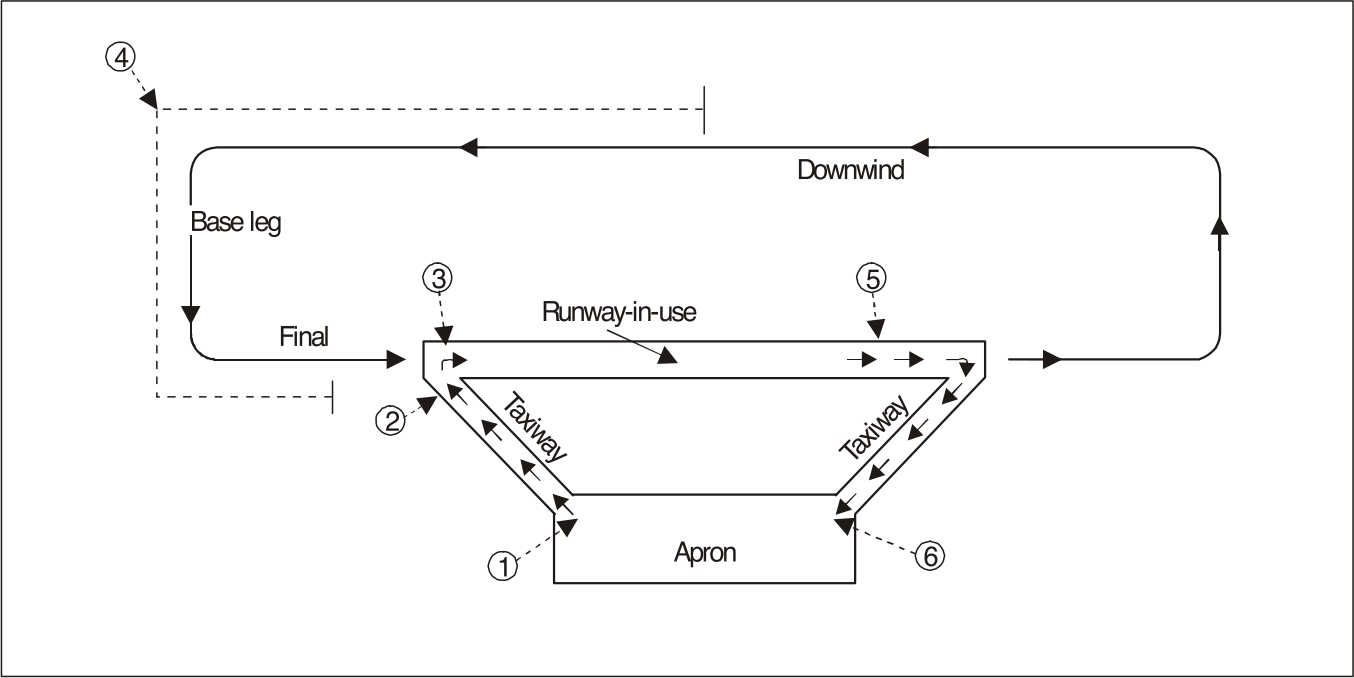
\includegraphics[width=14cm]{Images/Fig 7-1.png}
    \caption[Designated positions of aircraft from an aerodrome control tower viewpoint]{Designated positions of aircraft from an aerodrome control tower viewpoint (see \ref{7.6.2})}
    \label{fig:7-1}
\end{figure}

\subsubsection{Traffic on the manoeuvring area}

\begin{enumeratesc}
    \item \textsc{Control of taxiing aircraft}
    \begin{enumerate}[labelindent=0pt,itemsep=0.2cm]
        \item \textsc{Taxi clearance}
        \begin{enumerate}
            \item Prior to issuing a taxi clearance, the controller shall determine where the aircraft concerned is parked. Taxi clearances shall contain concise instructions and adequate information so as to assist the flight crew to follow the correct taxi routes, to avoid collision with other aircraft or objects and to minimize the potential for the aircraft inadvertently entering an active runway.
            \item When a taxi clearance contains a taxi limit beyond a runway, it shall contain an explicit clearance to cross or an instruction to hold short of that runway.
            \item The appropriate ATS authority should whenever practicable publish in the national AIP standard taxi routes to be used at an aerodrome. Standard taxi routes should be identified by appropriate designators and should be used in taxi clearances.
            \item Where standard taxi routes have not been published, a taxi route should, whenever possible, be described by use of taxiway and runway designators. Other relevant information, such as an aircraft to follow or give way to, shall also be provided to a taxiing aircraft.
        \end{enumerate}

        \item \textsc{Taxiing on a runway-in-use}
        \begin{enumerate}
            \item For the purpose of expediting air traffic, aircraft may be permitted to taxi on the runway-in-use, provided no delay or risk to other aircraft will result. Where control of taxiing aircraft is provided by a ground controller and the control of runway operations by an aerodrome controller, the use of a runway by taxiing aircraft shall be coordinated with and approved by the aerodrome controller. Communication with the aircraft concerned should be transferred from the ground controller to the aerodrome controller prior to the aircraft entering the runway.
            \item \label{7.6.3.1.2.2} If the control tower is unable to determine, either visually or via an ATS surveillance system that a vacating or crossing aircraft has cleared the runway, the aircraft shall be requested to report when it has vacated the runway. The report shall be made when the entire aircraft is beyond the relevant runway-holding position.
        \end{enumerate}

        \item \textsc{Use of runway-holding positions}
        \begin{enumerate}
            \item Except as provided in \ref{7.6.3.1.3.2} or as prescribed by the appropriate ATS authority, aircraft shall not be held closer to a runway-in-use than at a runway-holding position.
            \note{Runway-holding position locations in relation to runways are specified in Annex 14, Volume I, Chapter 5.}
            \item \label{7.6.3.1.3.2} Aircraft shall not be permitted to line up and hold on the approach end of a runway-in-use whenever another aircraft is effecting a landing, until the landing aircraft has passed the point of intended holding.
            \note{See Figure \ref{fig:7-2}.}
        \end{enumerate}

        %Figure 7-2
        \vspace{0.5cm}
        \begin{figure}[!ht]
            \centering
            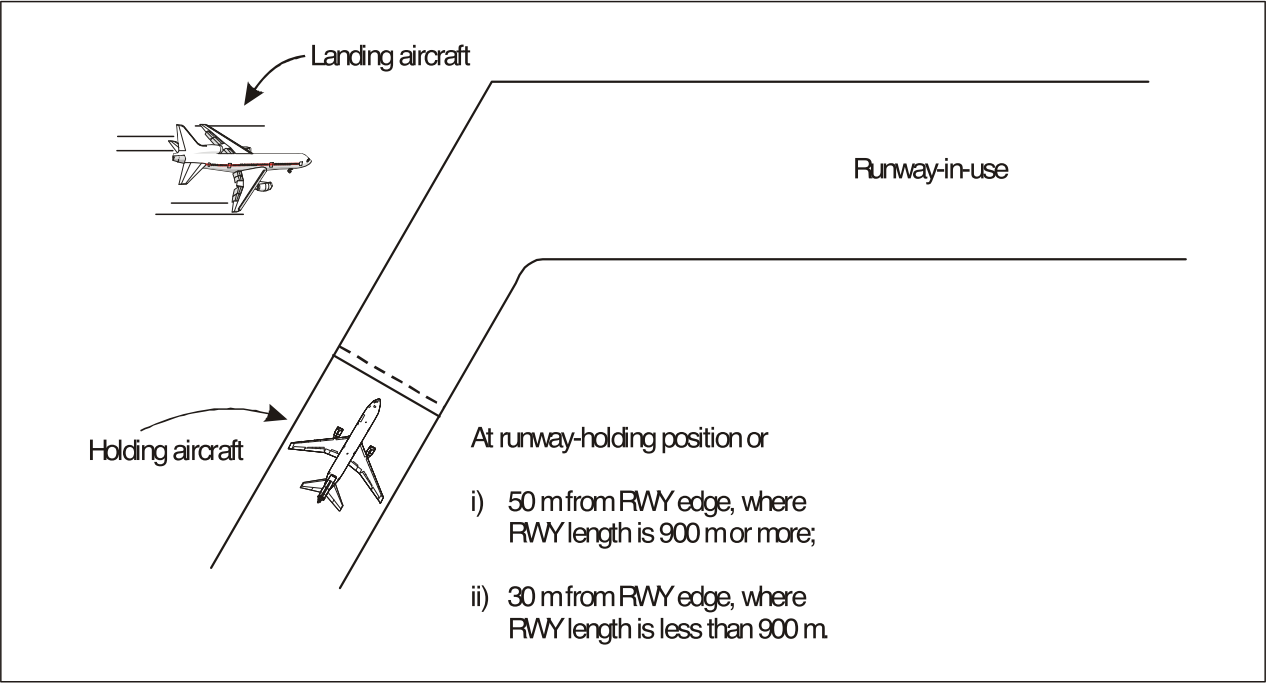
\includegraphics[width=14cm]{Images/Fig 7-2.png}
            \caption[Method of holding aircraft]{Method of holding aircraft (see \ref{7.6.3.1.3.2})}
            \label{fig:7-2}
        \end{figure}

        \item \textsc{Helicopter taxiing operations}
        \begin{enumerate}
            \item When necessary for a wheeled helicopter or vertical take-off and landing (VTOL) aircraft to taxi on the surface, the following provisions are applicable.
            \note{Ground taxiing uses less fuel than air-taxiing and minimizes air turbulence. However, under certain conditions, such as rough, soft or uneven terrain, it may become necessary to air-taxi for safety considerations. Helicopters with articulating rotors (usually designs with three or more main rotor blades) are subject to ``ground resonance" and may, on rare occasions, suddenly lift off the ground to avoid severe damage or destruction.}
            \item When it is requested or necessary for a helicopter to proceed at a slow speed above the surface, normally below 20 kt and in ground effect, air-taxiing may be authorized.
            \note{Air-taxiing consumes fuel at a high burn rate, and helicopter downwash turbulence (produced in ground effect) increases significantly with larger and heavier helicopters.}
            \item Instructions which require small aircraft or helicopters to taxi in close proximity to taxiing helicopters should be avoided and consideration should be given to the effect of turbulence from taxiing helicopters on arriving and departing light aircraft.
            \item A frequency change should not be issued to single-pilot helicopters hovering or air-taxiing. Whenever possible, control instructions from the next ATS unit should be relayed as necessary until the pilot is able to change frequency.
            \note{Most light helicopters are flown by one pilot and require the constant use of both hands and feet to maintain control during low-altitude/low-level flight. Although flight control friction devices assist the pilot, changing frequency near the ground could result in inadvertent ground contact and consequent loss of control.}
        \end{enumerate}
    \end{enumerate}

    % 7.6.3.2
\end{enumeratesc}

\subsection[Control of traffic in the traffic circuit]{CONTROL OF TRAFFIC IN THE TRAFFIC CIRCUIT}

\subsubsection{General}

\begin{enumerate}
    %References
    \item Aircraft in the traffic circuit shall be controlled to provide the separation minima outlined in \ref{7.9.2}, \ref{7.10.1} and \ref{7.11} and Chapter 5, Section 5.8, except that:

    \begin{enumalph}
        \item aircraft in formation are exempted from the separation minima with respect to separation from other aircraft of the same flight;
        \item aircraft operating in different areas or different runways on aerodromes suitable for simultaneous landings or take-offs are exempted from the separation minima;
        %References
        \item separation minima shall not apply to aircraft operating under military necessity in accordance with Chapter 16, Section 16.1.
    \end{enumalph}

    %References
    \item Sufficient separation shall be effected between aircraft in flight in the traffic circuit to allow the spacing of arriving and departing aircraft as outlined in \ref{7.9.2}, \ref{7.10.1} and \ref{7.11} and Chapter 5, Section 5.8.
\end{enumerate}

\subsubsection{Entry of traffic circuit}

\begin{enumerate}
    \item The clearance to enter the traffic circuit should be issued to an aircraft whenever it is desired that the aircraft approach the landing area in accordance with current traffic circuits but traffic conditions do not yet allow a landing clearance to be issued. Depending on the circumstances and traffic conditions, an aircraft may be cleared to join at any position in the traffic circuit.
    \item An arriving aircraft executing an instrument approach shall normally be cleared to land straight in unless visual manoeuvring to the landing runway is required.
\end{enumerate}

\subsubsection{Priority for landing}

\begin{enumerate}
    \item If an aircraft enters an aerodrome traffic circuit without proper authorization, it shall be permitted to land if its actions indicate that it so desires. If circumstances warrant, aircraft which are in contact with the controller may be instructed by the controller to give way so as to remove as soon as possible the hazard introduced by such unauthorized operation. In no case shall permission to land be withheld indefinitely.
    \item In cases of emergency it may be necessary, in the interests of safety, for an aircraft to enter a traffic circuit and effect a landing without proper authorization. Controllers should recognize the possibilities of emergency action and render all assistance possible.
    \item Priority shall be given to:

    \begin{enumalph}
        \item an aircraft which anticipates being compelled to land because of factors affecting the safe operation of the aircraft (engine failure, shortage of fuel, etc.);
        \item hospital aircraft or aircraft carrying any sick or seriously injured persons requiring urgent medical attention;
        \item aircraft engaged in search and rescue operations; and
        \item other aircraft as may be determined by the appropriate authority.
    \end{enumalph}

    %References
    \note{An aircraft which has encountered an emergency is handled as outlined in Chapter 15, Section 15.1.}
\end{enumerate}

\subsection[Order of priority for arriving and departing aircraft]{ORDER OF PRIORITY FOR ARRIVING AND DEPARTING AIRCRAFT}

An aircraft landing or in the final stages of an approach to land shall normally have priority over an aircraft intending to depart from the same or an intersecting runway.

\subsection[Control of departing aircraft]{CONTROL OF DEPARTING AIRCRAFT}

\subsubsection{Departure sequence}

Departures shall normally be cleared in the order in which they are ready for take-off, except that deviations may be made from this order of priority to facilitate the maximum number of departures with the least average delay. Factors which should be considered in relation to the departure sequence include, \textit{inter alia}:

\begin{enumalph}
    \item types of aircraft and their relative performance;
    \item routes to be followed after take-off;
    \item any specified minimum departure interval between take-offs;
    \item need to apply wake turbulence separation minima;
    \item aircraft which should be afforded priority; and
    \item aircraft subject to ATFM requirements.
\end{enumalph}

%References
\note[1]{See also Chapter 6, 6.3.3.}
\note[2]{For aircraft subject to ATFM requirements, it is the responsibility of the pilot and the operator to ensure that the aircraft is ready to taxi in time to meet any required departure time, bearing in mind that once a departure sequence is established on the taxiway system, it can be difficult, and sometimes impossible, to change the order.}

\subsubsection{Separation of departing aircraft} \label{7.9.2}

%References
Except as provided in \ref{7.11} and Chapter 5, Section 5.8, a departing aircraft will not normally be permitted to commence take-off until the preceding departing aircraft has crossed the end of the runway-in-use or has started a turn or until all preceding landing aircraft are clear of the runway-in-use.
\note[1]{See Figure \ref{fig:7-3}.}
%References
\note[2]{Wake turbulence categories and time-based wake turbulence longitudinal separation minima are contained in Chapter 4, Section 4.9 and Chapter 5, Section 5.8, respectively. Distance-based wake turbulence separation minima are contained in Chapter 8, Section 8.7.}
\note[3]{See \ref{7.6.3.1.2.2}.}

%Figure 7-3
\vspace{0.5cm}
\begin{figure}[!ht]
    \centering
    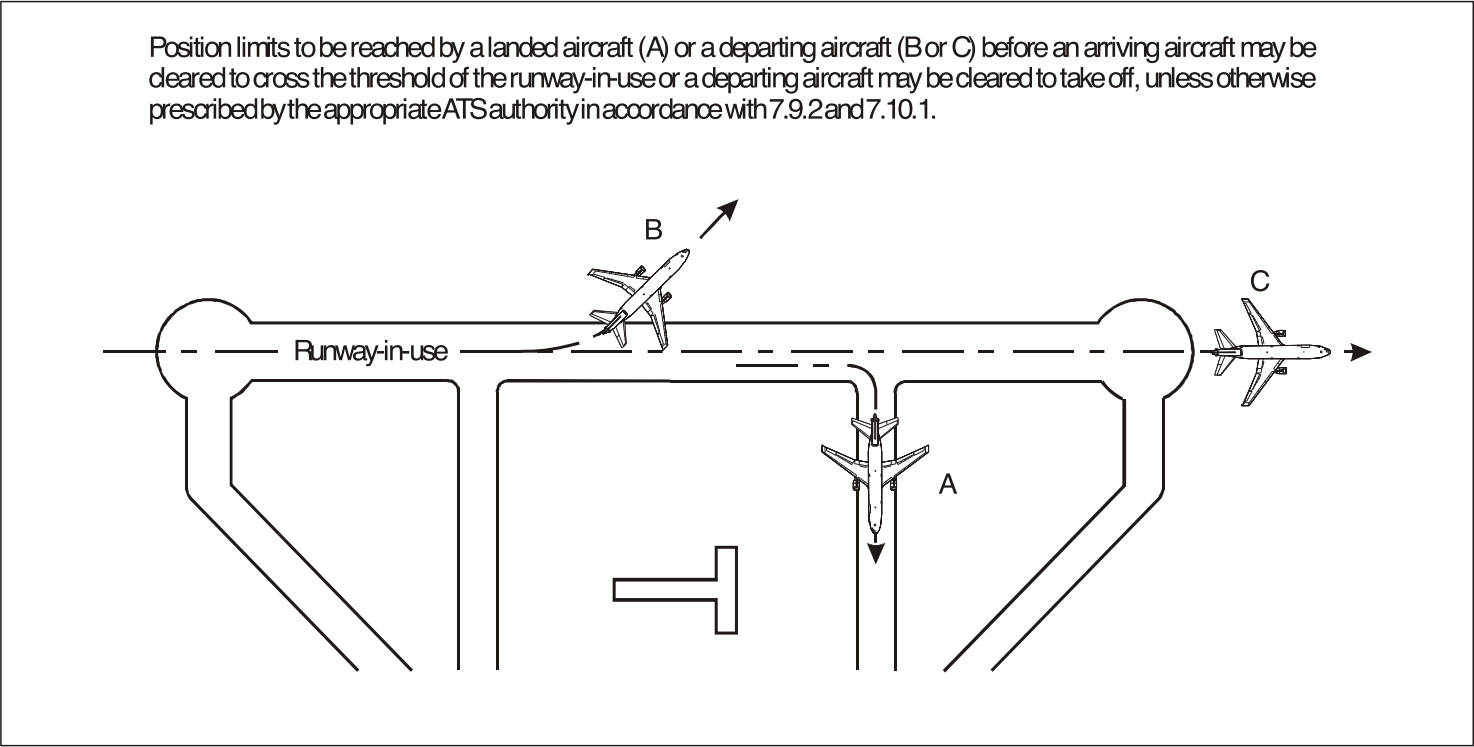
\includegraphics[width=14cm]{Images/Fig 7-3.png}
    \caption[Separation between departing and arriving aircraft]{Separation between departing and arriving aircraft (see \ref{7.9.2} and \ref{7.10.1})}
    \label{fig:7-3}
\end{figure}

\subsubsection{Take-off clearance}

\begin{enumerate}
    \item Take-off clearance may be issued to an aircraft when there is reasonable assurance that the separation in \ref{7.9.2}, or prescribed in accordance with \ref{7.11}, will exist when the aircraft commences take-off.
    \item \label{7.9.3.2} When an ATC clearance is required prior to take-off, the take-off clearance shall not be issued until the ATC clearance has been transmitted to and acknowledged by the aircraft concerned. The ATC clearance shall be forwarded to the aerodrome control tower with the least possible delay after receipt of a request made by the tower or prior to such request if practicable.
    \item The expression TAKE-OFF shall only be used in radiotelephony when an aircraft is cleared for take-off or when cancelling a take-off clearance.
    \note{The expression TORA, pronounced TOR-AH, may be used to indicate take-off run available.}
    \item Subject to \ref{7.9.3.2}, the take-off clearance shall be issued when the aircraft is ready for take-off and at or approaching the departure runway, and the traffic situation permits. To reduce the potential for misunderstanding, the take-off clearance shall include the designator of the departure runway.
    \item In the interest of expediting traffic, a clearance for immediate take-off may be issued to an aircraft before it enters the runway. On acceptance of such clearance the aircraft shall taxi out to the runway and take off in one continuous movement.
\end{enumerate}

\subsection[Control of arriving aircraft]{CONTROL OF ARRIVING AIRCRAFT}

\subsubsection[Separation of landing aircraft and preceding landing and departing aircraft using the same runway]{Separation of landing aircraft and preceding landing \\ and departing aircraft using the same runway} \label{7.10.1}

%References
Except as provided in \ref{7.11} and Chapter 5, Section 5.8, a landing aircraft will not normally be permitted to cross the runway threshold on its final approach until the preceding departing aircraft has crossed the end of the runway-in-use, or has started a turn, or until all preceding landing aircraft are clear of the runway-in-use.
\note[1]{See Figure \ref{fig:7-3}.}
%References
\note[2]{Wake turbulence categories of aircraft and longitudinal separation minima are contained in Chapter 4, Section 4.9 and Chapter 5, Section 5.8, respectively.}
\note[3]{See \ref{7.6.3.1.2.2}.}

\subsubsection{Clearance to land}

An aircraft may be cleared to land when there is reasonable assurance that the separation in \ref{7.10.1}, or prescribed in accordance with \ref{7.11} will exist when the aircraft crosses the runway threshold, provided that a clearance to land shall not be issued until a preceding landing aircraft has crossed the runway threshold. To reduce the potential for misunderstanding, the landing clearance shall include the designator of the landing runway.

\subsubsection{Landing and roll-out manoeuvres}

\begin{enumerate}
    \item When necessary or desirable in order to expedite traffic, a landing aircraft may be requested to:

    \begin{enumalph}
        \item hold short of an intersecting runway after landing;
        \item land beyond the touchdown zone of the runway;
        \item vacate the runway at a specified exit taxiway;
        \item expedite vacating the runway.
    \end{enumalph}

    \item In requesting a landing aircraft to perform a specific landing and/or roll-out manoeuvre, the type of aircraft, runway length, location of exit taxiways, reported braking action on runway and taxiway, and prevailing meteorological conditions shall be considered. A HEAVY aircraft shall not be requested to land beyond the touchdown zone of a runway.
    \item If the pilot-in-command considers that he or she is unable to comply with the requested operation, the controller shall be advised without delay.
    \item When necessary or desirable, e.g. due to low visibility conditions, a landing or a taxiing aircraft may be instructed to report when a runway has been vacated. The report shall be made when the entire aircraft is beyond the relevant runway-holding position.
\end{enumerate}

\subsection[Reduced runway separation minima between aircraft using the same runway]{REDUCED RUNWAY SEPARATION MINIMA BETWEEN \\ AIRCRAFT USING THE SAME RUNWAY} \label{7.11}

\begin{enumnoss}
    \item Provided that an appropriate, documented safety assessment has shown that an acceptable level of safety can be met, lower minima than those in \ref{7.9.2} and \ref{7.10.1} may be prescribed by the appropriate ATS authority, after consultation with the operators. The safety assessment shall be carried out for each runway for which the reduced minima are intended, taking into account factors such as:

    \begin{enumalph}
        \item runway length;
        \item aerodrome layout; and
        \item types/categories of aircraft involved.
    \end{enumalph}

    \item All applicable procedures related to the application of reduced runway separation minima shall be published in the Aeronautical Information Publication as well as in local air traffic control instructions. Controllers shall be provided with appropriate and adequate training in the use of the procedures.
    \item Reduced runway separation minima shall only be applied during the hours of daylight from 30 minutes after local sunrise to 30 minutes before local sunset.
    \item For the purpose of reduced runway separation, aircraft shall be classified as follows:

    \begin{enumalph}
        \item \textit{Category 1 aircraft:} single-engine propeller aircraft with a maximum certificated take-off mass of 2 000 kg or less;
        \item \textit{Category 2 aircraft:} single-engine propeller aircraft with a maximum certificated take-off mass of more than 2 000 kg but less than 7 000 kg; and twin-engine propeller aircraft with a maximum certificated take-off mass of less than 7 000 kg;
        \item \textit{Category 3 aircraft:} all other aircraft.
    \end{enumalph}

    \item Reduced runway separation minima shall not apply between a departing aircraft and a preceding landing aircraft.
    \item Reduced runway separation minima shall be subject to the following conditions:

    \begin{enumalph}
        \item wake turbulence separation minima shall be applied;
        \item visibility shall be at least 5 km and ceiling shall not be lower than 1 000 ft;
        \item tailwind component shall not exceed 5 kt;
        \item there shall be available means, such as suitable landmarks, to assist the controller in assessing the distances between aircraft. A surface surveillance system that provides the air traffic controller with position information on aircraft may be utilized, provided that approval for operational use of such equipment includes a safety assessment to ensure that all requisite operational and performance requirements are met;
        \item minimum separation continues to exist between two departing aircraft immediately after take-off of the second aircraft;
        \item traffic information shall be provided to the flight crew of the succeeding aircraft concerned; and
        \item the braking action shall not be adversely affected by runway contaminants such as ice, slush, snow and water.
    \end{enumalph}

    \item Reduced runway separation minima which may be applied at an aerodrome shall be determined for each separate runway. The separation to be applied shall in no case be less than the following minima:

    \begin{enumalph}
        \item landing aircraft:
        \begin{enumarab}
            \item a succeeding landing Category 1 aircraft may cross the runway threshold when the preceding aircraft is a Category 1 or 2 aircraft which either:

            \begin{enumroman}
                \item has landed and has passed a point at least 600 m from the threshold of the runway, is in motion and will vacate the runway without backtracking; or
                \item is airborne and has passed a point at least 600 m from the threshold of the runway;
            \end{enumroman}

            \item a succeeding landing Category 2 aircraft may cross the runway threshold when the preceding aircraft is a Category 1 or 2 aircraft which either:

            \begin{enumroman}
                \item has landed and has passed a point at least 1 500 m from the threshold of the runway, is in motion and will vacate the runway without backtracking; or
                \item is airborne and has passed a point at least 1 500 m from the threshold of the runway;
            \end{enumroman}

            \item a succeeding landing aircraft may cross the runway threshold when a preceding Category 3 aircraft:

            \begin{enumroman}
                \item has landed and has passed a point at least 2 400 m from the threshold of the runway, is in motion and will vacate the runway without backtracking; or
                \item is airborne and has passed a point at least 2 400 m from the threshold of the runway;
            \end{enumroman}
        \end{enumarab}

        \item departing aircraft:
        \begin{enumarab}
            \item a Category 1 aircraft may be cleared for take-off when the preceding departing aircraft is a Category 1 or 2 aircraft which is airborne and has passed a point at least 600 m from the position of the succeeding aircraft;
            \item a Category 2 aircraft may be cleared for take-off when the preceding departing aircraft is a Category 1 or 2 aircraft which is airborne and has passed a point at least 1 500 m from the position of the succeeding aircraft; and
            \item an aircraft may be cleared for take-off when a preceding departing Category 3 aircraft is airborne and has passed a point at least 2 400 m from the position of the succeeding aircraft.
        \end{enumarab}
    \end{enumalph}

    \begin{enumnoss}
        \item Consideration should be given to increased separation between high performance single-engine aircraft and preceding Category 1 or 2 aircraft.
    \end{enumnoss}
\end{enumnoss}

\subsection[Procedures for low visibility operations]{PROCEDURES FOR LOW VISIBILITY OPERATIONS}

\subsubsection[Control of aerodrome surface traffic in conditions of low visibility]{Control of aerodrome surface traffic \\ in conditions of low visibility}

\begin{enumempty}[labelindent=\parindent]
    \item \note{These procedures apply whenever conditions are such that all or part of the manoeuvring area cannot be visually monitored from the control tower. Additional requirements which apply when category II/III approaches are being conducted are specified in Section \ref{7.12.2}.}
\end{enumempty}

\begin{enumerate}
    \item When there is a requirement for traffic to operate on the manoeuvring area in conditions of visibility which prevent the aerodrome control tower from applying visual separation between aircraft, and between aircraft and vehicles, the following shall apply:

    \begin{enumerate}
        \item At the intersection of taxiways, an aircraft or vehicle on a taxiway shall not be permitted to hold closer to the other taxiway than the holding position limit defined by a clearance bar, stop bar or taxiway intersection marking according to the specifications in Annex 14, Volume I, Chapter 5.
        \item The longitudinal separation on taxiways shall be as specified for each particular aerodrome by the appropriate ATS authority. This separation shall take into account the characteristics of the aids available for surveillance and control of ground traffic, the complexity of the aerodrome layout and the characteristics of the aircraft using the aerodrome.
    \end{enumerate}

    \note{The \emph{Manual of Surface Movement Guidance and Control Systems (SMGCS)} (Doc 9476) provides guidance on surface movement guidance and control components and procedures for low visibility operations.}
\end{enumerate}

\subsubsection[Procedures for control of aerodrome traffic when category II/III approaches are in use]{Procedures for control of aerodrome traffic \\ when category II/III approaches are in use} \label{7.12.2}

\begin{enumerate}
    \item The appropriate ATS authority shall establish provisions applicable to the start and continuation of precision approach category II/III operations as well as departure operations in RVR conditions less than a value of 550 m.
    \item Low visibility operations shall be initiated by or through the aerodrome control tower.
    \item The aerodrome control tower shall inform the approach control unit concerned when procedures for precision approach category II/III and low visibility operations will be applied and also when such procedures are no longer in force.
    \item Provisions regarding low visibility operations should specify:

    \begin{enumalph}
        \item the RVR value(s) at which the low visibility operations procedures shall be implemented;
        \item the minimum ILS/MLS equipment requirements for category II/III operations;
        \item other facilities and aids required for category II/III operations, including aeronautical ground lights, which shall be monitored for normal operation;
        \item the criteria for and the circumstances under which downgrading of the ILS/MLS equipment from category II/III operations capability shall be made;
        \item the requirement to report any relevant equipment failure and degradation, without delay, to the flight crews concerned, the approach control unit, and any other appropriate organization;
        \item special procedures for the control of traffic on the manoeuvring area, including:

        \begin{enumarab}
            \item the runway-holding positions to be used;
            \item the minimum distance between an arriving and a departing aircraft to ensure protection of the sensitive and critical areas;
            \item procedures to verify that aircraft and vehicles have vacated the runway;
            \item procedures applicable to the separation of aircraft and vehicles;
        \end{enumarab}

        \item applicable spacing between successive approaching aircraft;
        \item action(s) to be taken in the event low visibility operations need to be discontinued, e.g. due to equipment failures; and
        \item any other relevant procedures or requirements.
    \end{enumalph}

    \note{Further information regarding the requirements for low visibility operations can be found in the \emph{Air Traffic Services Planning Manual} (Doc 9426) and the \emph{All-Weather Operations Manual} (Doc 9365).}

    % 7.12.6 
\end{enumerate}

\subsection[Suspension of visual flight rules operations]{SUSPENSION OF VISUAL FLIGHT RULES OPERATIONS}

\begin{enumnoss}
    \item Any or all VFR operations on and in the vicinity of an aerodrome may be suspended by any of the following units, persons or authorities whenever safety requires such action:

    \begin{enumalph}
        \item the approach control unit or the appropriate ACC;
        \item the aerodrome control tower;
        \item the appropriate ATS authority.
    \end{enumalph}

    \item All such suspensions of VFR operations shall be accomplished through or notified to the aerodrome control tower.
    \item The following procedures shall be observed by the aerodrome control tower whenever VFR operations are suspended:

    \begin{enumalph}
        \item hold all VFR departures;
        \item recall all local flights operating under VFR or obtain approval for special VFR operations;
        \item notify the approach control unit or ACC as appropriate of the action taken;
        \item notify all operators, or their designated representatives, of the reason for taking such action, if necessary or requested.
    \end{enumalph}
\end{enumnoss}

\subsection[Authorization of special VFR flights]{AUTHORIZATION OF SPECIAL VFR FLIGHTS}

\begin{enumnoss}
    \item When traffic conditions permit, special VFR flights may be authorized subject to the approval of the unit providing approach control service and the provisions of \ref{7.14.1.3}.

    \begin{enumnoss}
        \item Requests for such authorization shall be handled individually.
        %References
        \item Separation shall be effected between all IFR flights and special VFR flights in accordance with separation minima in Chapters 5 and 6 and, when so prescribed by the appropriate ATS authority, between all special VFR flights in accordance with separation minima prescribed by that authority.
        \item \label{7.14.1.3} When the ground visibility is not less than 1 500 m, special VFR flights may be authorized to: enter a control zone for the purpose of landing, take off and depart from a control zone, cross a control zone or operate locally within a control zone.
    \end{enumnoss}

    \note{Requirements for two-way communications between controlled flights and the appropriate air traffic control unit are contained in Annex 2, 3.6.5.}
\end{enumnoss}

%Numbering
% 7.15 AERONAUTICAL GROUND LIGHTS

\subsection[Designation of hot spot(s)]{DESIGNATION OF HOT SPOT(S)}

%References
The aerodrome operator shall designate, whenever necessary, a location or several locations on the movement area of the aerodrome as hot spot(s). The hot spot(s) shall be charted in accordance with Annex 4, 13.6, 14.6, 15.6 and Appendix 2.
\note{Guidance material related to hot spots is contained in the \emph{Manual on the Prevention of Runway Incursions} (Doc 9870).}

\chapterend